\documentclass[letterpaper, 11pt]{article}
\usepackage[margin=1in, centering]{geometry}
\usepackage{sectsty}
\usepackage{graphicx}
\usepackage{here}
\usepackage{caption}
\usepackage{subcaption}
\usepackage{pdfpages}
\usepackage[export]{adjustbox}
\captionsetup{labelformat = empty}

% Formato: Ángel Alvarado Campos @Flutt

\begin{document}
	
	\begin{figure}[H] %Portada
		\begin{subfigure}{0.2\textwidth}
			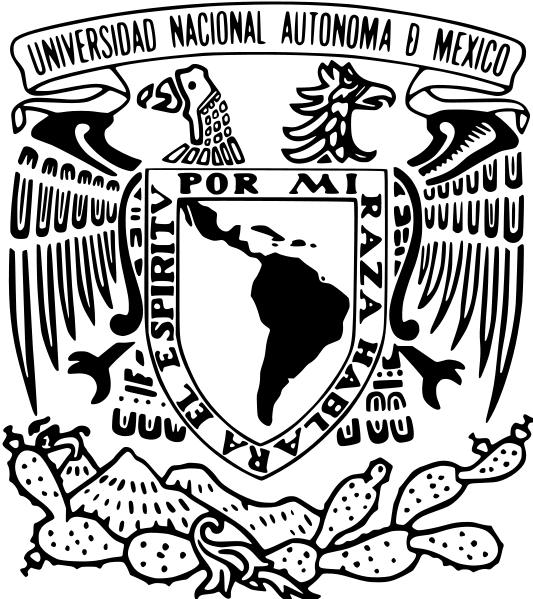
\includegraphics[scale = 0.16 ,left]{Imagenes/Portada/Escudo_UNAM.png}
		\end{subfigure}
		\hfill
		\begin{subfigure}{0.5\textwidth}
			\centering
			{\fontsize{15}{15} \selectfont Universidad Nacional Autónoma de México}
			
			\vspace{6mm}
			
			{\fontsize{15}{15} \selectfont Facultad de Ingeniería}
		\end{subfigure}
		\hfill
		\begin{subfigure}{0.2\textwidth}
			
\includegraphics[scale = 1, right]{Imagenes/Portada/Escudo_FI.jpg}
		\end{subfigure}
		
		\vspace{15mm}
		
		\centering
		{\fontsize{18}{18} \selectfont Estructuras de Datos y Algoritmos II}
		
		\vspace{25mm}
		
		{\fontsize{18}{18} \selectfont \textbf{Proyecto adicional: Árboles binarios}}
		
		\vspace{20mm}
		
		{\fontsize{15}{15} \selectfont \textbf{Presenta:}}\\
		{\fontsize{15}{15} \selectfont Alvarado Campos, Ángel}\\
		
		\vspace{25mm}
		
		{\fontsize{15}{15} \selectfont \textbf{Profesor:}}\\
		{\fontsize{15}{15} \selectfont Tista García, Edgar}\\
		
		\vspace{25mm}
		
		{\fontsize{15}{15} \selectfont \textbf{Semestre:}}\\
		{\fontsize{15}{15} \selectfont 2021-1}\\
	\end{figure} %Fin Portada
	\pagestyle{empty}
	\newpage
	
	\section*{\centering 0bjetivo}
		Que el alumno implemente árboles binarios y que desarrolle sus habilidades de la programación orientada a objetos a través de la aplicación del concepto de árboles como estructuras de datos no lineales. \\
		
		Que el alumno obtenga una mayor comprensión técnica y conceptual de la lógica detrás de algunas implementaciones de árbol binario.
		
	\section*{\centering Marco teórico}
	
	En Ciencias de la Computación, se le llama árbol a una estructura de datos no lineal y recursiva, formada por interacciones entre pequeñas estructuras autoreferenciales llamadas nodos, los cuales pueden tener referencias a otros nodos o no. 
	
	En particular, llama la atención y es objeto de estudio de este proyecto un tipo de árbol llamado árbol binario, el cual cumple con la propiedad de que para todos los nodos referenciados, se tiene a lo mucho dos nodos hijos. Por si sóla, una estructura de árbol binario no tiene mucho que ofrecer, pero las distintas implementaciones y aplicaciones de ésta son las que obtienen el máximo provecho de sus propiedades. 
	
	En este proyecto se estudian y presentan tres implementaciones importantes de árbol binario: arbol binario de búsqueda autobalanceado, árbol binario de expresión aritmética, y \textit{heap}. En las siguientes lineas de describen los conceptos básicos para la comprensión de este proyecto.
	
	\subsection*{Árbol binario de búsqueda y concepto de autobalanceo}
	
	Un árbol binario de búsqueda es un tipo de árbol binario en el que ser verifica que cada uno de los nodos involucrados en el sistema tengan un hijo izquierdo con una clave menor y un hijo derecho con una clave mayor. En otras palabras, para todos los nodos, el subárbol izquierdo contiene claves con menor valor y el subárbol derecho contiene claves mayor valor. 
	
	En esencia, un árbol de binario de búsqueda es una de las mejores implementaciones de para algoritmos de búsqueda, sin embargo, esto solo se mantiene para el caso promedio o mejor caso, pues en el peor caso se tendrá una complejidad lineal; proporcional a la búsqueda en una lista secuencial. 
	
	En este punto conviene mencionar el concepto de nivel de un árbol. Dado un árbol, si se considera que el nodo raíz de la estructura tiene un nivel 0, entonces sus hijos tienen el nivel 1, sus nietos el nivel 2, y así sucesivamente. Resulta evidente entonces que mientras todos los nodos tengan menor diferencia de niveles entre sus subárboles, mejor rendimiento tendrá la estructura.
	
	El concepto de balanceo consiste en una estructura de árbol binario de búsqueda que mantenga un mejor rendimiento a través de la búsqueda de la mejor disposición de nodos, tal que exista una menor diferencia de nivel entre los subárboles de cada nodo involucrado. En cuanto al autobalanceo, se trata una implementación de árbol binario que se mantenga balanceada tras cada operación de inserción o eliminación.
	
	\subsection*{Árbol binario semicompleto y \textit{heap}}
	
	Un árbol binario semicompleto es un árbol binario (no de búsqueda) en el que todos los niveles relacionados están completos a excepción del último. En este último nivel todos los nodos deben aparecer de izquierda a derecha, es decir, por cada nivel incompleto se debe realizar la colocación de nodos de izquierda a derecha.
	
	Por otro lado, una estructura de montículo o \textit{heap} se trata de un árbol binario semicompleto en el que se cumple la propiedad de que el valor de cada nodo es mayor que el de sus hijos, de manera recursiva. El caso mencionado se trata de un \textit{heap} de máxima, sin embargo, también existen los \textit{heap} de mínima, en los que se cumple la propiedad de manera inversa, es decir, que el valor de cada nodo es menor que el sus hijos.
	
	En este proyecto, la implementación de \textit{heap} presentada corresponde a un \textit{heap} de máxima.
	
	\subsection*{Árbol binario de expresiones aritméticas}
	
	Los árboles binarios de expresiones aritméticas son, en sí, aplicaciones de lo árboles binarios, pues permiten resolver expresiones aritméticas lineales por medio de la disposición de la expresión en un árbol binario. 
	
	Las reglas para representar una expresión aritmética mediante un árbol binario son las siguientes:
	
	\begin{enumerate}
		\item Cada nodo hoja contiene a un operando.
		\item Cada nodo intermedio (cada nodo que es padre) contiene a un operador.
	\end{enumerate}

	Una vez que se tiene a dicho árbol se puede ejecutar algún algoritmo para resolver la expresión. En este proyecto se solicitó implementar el algoritmo de la notación polaca inversa, la cual consiste en obtener la notación postfija del árbol y resolver con ayuda de una pila auxiliar. Esto se explica con mayor detalle en la sección que corresponde al desarrollo del proyecto.
	
	\section*{\centering Desarrollo}
	
	A continuación se describe el proceso de desarrollo de cada una de las estructuras implementadas, así como algunos detalles técnicos relevantes en cada de una de éstas.
	
	Antes de especificar en qué consiste cada estructura, es importante mencionar algunos aspectos generales que se comparten en grandes regiones del código. En primer lugar, las tres estructuras propuestas se definieron como subclases de una clase abstracta "ArbolBinario". Esta clase tiene como único atributo a un objeto de la clase "Nodo", el cual denota al nodo raíz o padre de todo la estructura.
	
	La clase "Nodo" es la estructura atómica y fundamental para la creación y operación de las subclases que heredan de "ArbolBinario". Se trata de una estructura autoreferencial que contiene cuatro atributos: tres de la clase "Nodo", tal que dos de ellos representan a sus hijos (nodo izquierdo y nodo derecho) y otro a su nodo padre; y a un objeto de la clase general "Object" que se refiere al dato que contiene el nodo. En la misma clase "Nodo" también se definen los \textit{getters} y \textit{setters} para cada uno de los atributos de la estructura, y se define un método constructor no vacío, el cual recibe como argumento a algún objeto de la clase "Object" y lo asigna al atributo que corresponde; además, en este mismo se método se hacen nulas las referencias de los nodos hijos, de tal manera que cada nodo creado es independiente por si mismo hasta que indique lo contrario en un proceso de adición de nodos. 
	
	Continuando con la clase abstracta, éste únicamente contiene dos métodos que conviene mencionar: "Print" y "Menu". "Print" es un método definido (no abstracto) el cual se encarga de imprimir en pantalla a cualquier estructura de árbol que herede de la clase abstracta, mientras que "Menu" sí es un método abstracto que es declarado para que cada subclase defina su menú de interacción con el usuario. En un inicio se consideró declarar como abstractos a los métodos de adición, eliminación, búsqueda, etc. como métodos generales (abstractos) de la clase "ArbolBinario" para que se pudiera hacer uso de polimorfismo y reducir sentencias de código, sin embargo, ya que cada estructura cuenta con operaciones únicas que no se pueden generalizar fácilmente (sin contar a la operación de impresión), se decidió declarar al método abstracto "Menu" para que cada estructura pudiera definir un conjunto de operaciones que puedan ser accedidas desde ese método y desde alguna otra región del sistema. \\
	
	Gran parte de este trabajo (sobre todo en la estructura de árbol binario autobalanceado) tomó como base a las prácticas 8 y 9 de la asignatura, pues en las entregas realizadas se desarrollaron algunos métodos robustos que se presentan también en este proyecto.
	
	\subsection*{Árbol binario autobalanceado}
	
	La implementación de árbol binario autobalanceado llevada a cabo en este proyecto se basó en la conocida estructura de árbol AVL. No se puede afirmar que es la misma implementación, pues la que se desarrolló no profundiza en el aspecto de las rotaciones de árbol dada la complejidad que representó plantear este movimiento en la estructura. 
	En lugar de las rotaciones planteadas en la estructura AVL, se contempló una forma diferente para efectuar la operación de balanceo. Convendría realizar algún análisis de complejidad para conocer la eficiencia de la estructura planteada, pues el código que se presenta no ésta basado en alguna bibliografía y se desconoce si ha sido propuesta anteriormente.
	
	Esta estructura es bastante similar a la de un árbol binario de búsqueda ordinario, pues mantiene la misma dinámica de adición y eliminación de nodos. El cambio se presenta cuando se realiza una operación que implica la modificación de la estructura; pues cuando se presenta una situación de esa naturaleza, se realiza una llamada a un método llamado "balancear". 
	
	Los métodos de adición y eliminación son, en esencia, los mismos de una implementación de árbol binario de búsqueda, y ya que esta estructura se desarrolló en las prácticas 8 y 9 de la asignatura, en este reporte no se describen a dichas funciones. En su lugar, conviene describir al método de balanceo propuesto, pues éste es la diferencia entre ambas estructuras.
	
	\begin{figure}[H]
		\centering
		\includegraphics[scale=0.5]{"Imagenes/Método balancear"}
		\caption{Método "balancear"}
	\end{figure}
	 
	 El método "balancear" tiene tipo de retorno "Nodo" y es llamado cuando se realiza una adición o eliminación de nodos idéntica a la de los árboles binarios de búsqueda ordinarios. Al finalizar la ejecución de este método, se retorna una referencia a un nodo raíz de algún árbol que cuenta con los mismos nodos del árbol original, pero en una estructura balanceada.
	 
	 El método en cuestión recibe como argumento a un objeto de la clase "Nodo", el cual es el padre de la estructura que se desea balancear; por lo tanto, resulta evidente que el argumento de este método siempre será el nodo raíz del árbol operado. Dentro del método se crea una instancia de "ArrayList" con elementos enteros y se realiza alguna llamadas especiales a ciertos métodos.
	 
	 Como se observa en la imagen anterior, los dos métodos auxiliares de "balancear" son "ListaOrdenada" y "Array\_a\_Arbol". El primero es llamado inmediatamente ante la creación de la instancia de "ArrayList" y recibe como argumento al nodo padre de la estructura y a la colección mencionada. Lo que se realiza en este método es almacenar en la colección de tipo "ArrayList" a todas las claves del árbol, ordenadas de menor a mayor, cuya raíz es el nodo argumentado. Ya que en el momento en que se aplica este método, la estructura es un árbol binario de búsqueda no balanceado (obligatoriamente), se puede aplicar el recorrido por inorden para obtener a todas las claves en un orden de menor a mayor. Resulta que el método "ListaOrdenada" realiza el recorrido por inorden para concluir con una colección que contiene a todas las claves del árbol ordenadas de menor mayor.
	 
	 Finalmente, se realiza una llamada al método "Array\_a\_Arbol" y se retorna a la referencia de "Nodo" dada por éste (dicha referencia es la que se mencionó anteriormente). El método "Array\_a\_Arbol" es un método de naturaleza recursiva que recibe como argumentos a una colección de tipo "ArrayList" de enteros que se quiere repartir en un árbol binario de manera balanceada, y a dos valores enteros que denotan los índices menores y mayores de la colección que se repartirán en una recursión, respectivamente. 
	 
	 Si se tiene una lista de elementos enteros ordenados de menor a mayor, de izquierda a derecha, y ésta se parte a la mitad, se sabe que la sublista que queda del lado izquierdo tiene únicamente elementos menores, mientras que el lado derecho tiene elementos mayores, respecto al elemento medio en que se tomó la partición. Si se aplica este proceso para cada sublista de manera recursiva, y se toma a cada elemento medio como indice padre, y a sus hijos izquierdo y derecho como el padre de la sublista izquierda y derecho, respectivamente, al final se tendrá una estructura casi simétrica y balanceada. Lo anterior es el fundamento conceptual de esta implementación de árbol binario balanceado.
	 
	 De lo anterior, se puede entender facilmente la razón de la naturaleza recursiva del método "Array\_a\_Arbol".
	 
	 \begin{figure}[H]
	 	\centering
	 	\includegraphics[scale=0.5]{"Imagenes/Método Array a Arbol"}
	 	\caption{Método "Array\_a\_Arbol"}
	 \end{figure}
	 
	Para probar a la estructura creada, se tiene el siguiente ejemplo de un árbol binario de búsqueda no balanceado.
	
	\begin{figure}[H]
		\centering
		\includegraphics[scale=0.3]{"Imagenes/ABB no balanceado"}
		\caption{ABB no balanceado}
	\end{figure}
	
	Al ejecutar el programa y asignar una secuencia de adiciones equivalentes, se obtuvo la siguiente impresión en pantalla.
	
	\begin{figure}[H]
		\centering
		\includegraphics[scale=0.5]{"Imagenes/ABB balanceado 1"}
		\caption{}
		\label{fig:abb-balanceado-1}
	\end{figure}
	
	Lo anterior describe al siguiente árbol y, por lo tanto, se comprueba que el programa cumple con la funcionalidad de balancear al árbol y que éste conserve las propiedades de un árbol binario de búsqueda.
	
	\begin{figure}[H]
		\centering
		\includegraphics[scale=0.3]{"Imagenes/ABB balanceado 2"}
		\caption{ABB balanceado}
	\end{figure}
	
	Por otro lado, si se efectúa la eliminación del nodo raíz, es decir, de aquel con clave 23, se obtiene la siguiente impresión en pantalla.
	
	\begin{figure}[H]
		\centering
		\includegraphics[scale=0.5]{"Imagenes/ABB balanceado Eliminación 1"}
		\caption{Eliminación del nodo 23}
	\end{figure}
	
	Las impresiones describen al siguiente árbol de búsqueda, y se reitera el correcto funcionamiento del algoritmo.
	
	\begin{figure}[H]
		\centering
		\includegraphics[scale=0.3]{"Imagenes/ABB balanceado Eliminación 2"}
		\caption{Representación gráfica del árbol después de la eliminación}
	\end{figure}
	
	\subsection*{\textit{heap}}
	
	La implementación de \textit{heap} desarrollada para este proyecto se basó en la definición de Sznajdleder en su obra \textit{Algoritmos a fondo}. En un inició se intentó realizar una implementación basada totalmente en los árboles binarios, es decir, haciendo uso únicamente de nodos y sus referencias; sin embargo, lo anterior no fue posible porque conservar la estructura de \textit{heap} implica reconocer las regiones donde se deben colocar los nuevos nodos, y para ello conviene utilizar algún complemento que brinde acceso global al sistema de nodos en general. 
	
	De cierta manera, a pesar de que fue muy complejo desarrollar a la estructura autobalanceable anterior, está fue más complicada por la situación mencionada. 
	
	La clase "Heap" que expresa a una estructura de datos de montículo, además de contar con el atributo estándar (nodo raíz) dado por la herencia de la clase "ArbolBinario", también cuenta con un atributo de tipo "ArrayList" con elementos enteros, tal que esta estructura proporciona un punto de acceso global a los nodos libres para realizar inserciones. Además, también se cuenta con un atributo entero llamado "elementos" el cual denota a la cantidad total de nodos en el árbol.
	
	La clase cuenta con un constructor vacío, en el cual, al nodo raíz se le asigna una referencia nula y a elementos se le inicializa en cero.
	
	El principal problema que se enfrentó en el desarrollo de esta estructura fue mantener la propiedad de árbol semicompleto, con inserciones de izquierda a derecha. Lo anterior se refiere a que si se tiene que insertar una clave como hija de un nodo, y el nodo hijo izquierdo está vacío, se le debe dar prioridad a ese nodo; pero en caso contrario se debe anexar la clave al hijo derecho. Esa situación parece facilmente programable, pero el problema surge cuando ambos nodos no están vacíos; esto implica que se debería realizar una búsqueda recursiva en ambos subárboles, para conocer la posición en la que se debe colocar la clave. 
	
	Ante la complejidad resultante de generalizar dicha situación, se tomó como referencia al arreglo de nodos y a la variable que indica el número de nodos en lista. Con la colección "ArrayList" descrita, se cuanta con la información de la cantidad total de nodos añadidos, por lo tanto, en función de esta cantidad se puede conocer el siguiente nodo disponible para añadir. El nodo padre del nuevo nodo (el que se va a añadir) se obtiene de la colección de nodos a través del índice dado por la función $f(e)=\frac{e-1}{2}$ donde $e$ denota la cantidad total de elementos previos a la adición. Dependiendo de los hijos que pueda tener dicho nodo padre, se podrá añadir el nodo nuevo fácilmente en la posición de hijo que le corresponde. 
	
	Para finalizar la adición, se presenta un método "AregarAux", el cual recibe como argumento al nodo recién agregado y se encarga de mantener la integridad del \textit{heap}. Ya que cada nodo tiene una referencia directa a su nodo padre, es posible verificar la integridad del \textit{heap} desde el nodo añadido hasta la raíz para recolocar a las claves involucradas.
	
	\begin{figure}[H]
		\centering
		\includegraphics[scale=0.5]{"Imagenes/Método de recolocación"}
		\caption{Método de recolocación de claves para mantener la integridad del \textit{heap}, "AgregarAux"}
	\end{figure}
	
	Una vez que concluya la adición, se realiza un incremento unitario a la variable "elementos".
	
	Por otro lado, la función de eliminación sólo está disponible para eliminar a la raíz de la estructura. En esencia, esta operación es inversa a la recolocación de claves de "AgregarAux", pues en este método se reemplaza a la clave de la raíz con la última clave anexada y se hace la verificación/recolocación desde la raíz hasta algún nodo donde se cumpla con la integridad. En este método, el primer paso es retirar de la colección de nodos al último nodo anexado, el cual coincide con el índice dado por la variable elementos menos 1. Una vez que se tiene a dicho nodo, se cortan las referencias involucradas con su nodo padre y se coloca la clave de éste nodo en el nodo raíz. 

	Posteriormente, con ayuda de un método recursivo llamado "EliminarRaizAux", se realiza la recolocación de claves, siempre y cuando el nodo en curso no sea un nodo hoja. \\
	
	Para probar a la estructura realizada se realizó una prueba con el ingreso de la siguiente secuencia de elementos enteros: $\{1,2,3,4,5,6,7,8,9,10\}$. Al ejecutar el programa se obtuvo la siguiente impresión en pantalla.
	
	\begin{figure}[H]
		\centering
		\includegraphics[scale=0.5]{"Imagenes/Heap 1"}
	\end{figure}
	
	Las impresiones describen a la siguiente estructura, y por lo tanto, se confirma la efectividad de la operación de adición en esta implementación de \textit{heap}.
	
	\begin{figure}[H]
		\centering
		\includegraphics[scale=0.3]{"Imagenes/Heap 2"}
		\caption{Representación gráfica del \textit{heap} después de añadir nodos}
	\end{figure}

	Por último, si se elimina la raíz una vez se obtiene la siguiente impresión en pantalla.
	
	\begin{figure}[H]
		\centering
		\includegraphics[scale=0.5]{"Imagenes/Heap eliminación"}
		\caption{}
	\end{figure}
	
	Las impresiones describen a la siguiente estructura, entonces se confirma la efectividad de la operación de eliminación de raíz en el \textit{heap}.
	
	\begin{figure}[H]
		\centering
		\includegraphics[scale=0.3]{"Imagenes/Heap eliminación 1"}
		\caption{Representación gráfica del \textit{heap} después de la eliminación de la raíz}
	\end{figure}
	
	\subsection*{Árbol de expresión aritmética}
	
	Esta estructura fue la más compleja de realizar y, de hecho, está inconclusa de cierta manera. El algoritmo presente sí funciona y permite realizar operaciones binarias, sin embargo, sólo lo puede hacer con números unitarios, es decir, aquellos formados por una sóla cifra. 
	
	El principal problema que se enfrentó al realizar esta implementación fue la lectura de una secuencia aritmética. En el momento en que se realizó el programa, se optó por recibir a la expresión aritmética como una cadena de tipo "String". Ésta es recibida como argumento en un método llamado "Lectura", en el cual se convierte a la cadena en un arreglo de caracteres y, posteriormente, con ayuda de un método de naturaleza recursiva llamado "LecturaAux", cuyo tipo de retorno es "Nodo", se construye el árbol de expresión aritmética y al nodo raíz se le asigna la referencia a dicho árbol. 
	
	En esencia, lo que se hace en el método "LecturaAux" es obtener el nodo padre de toda la estructura con ayuda del método "IndexAux". El valor de "IndexAux" proporcionará el índice del arreglo de expresión en el que está el nodo padre y, posteriormente, a los nodos hijos de éste, se les asigna de forma recursiva, el nodo dado por el mismo método "LecturaAux" pero ahora con los índices que corresponden al lado izquierdo de la expresión y al lado derecho a partir de la división dada por "IndexAux". El caso base de este método se da cuando se tienen como argumento del método a dos indices tales que la subexpresión a evaluar consta únicamente de dos elementos enteros y un operador.  
	
	\begin{figure}[H]
		\centering
		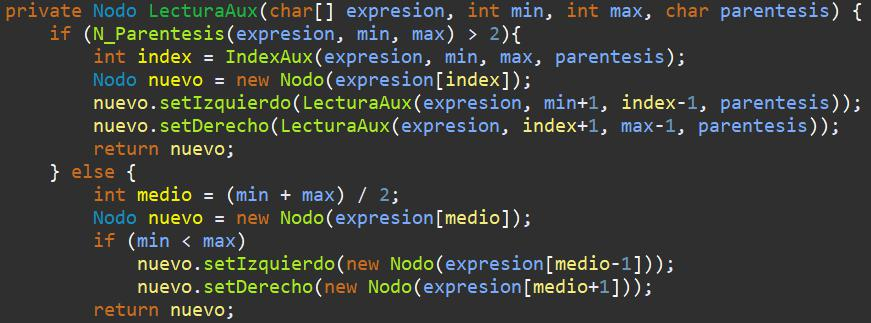
\includegraphics[scale=0.4]{Imagenes/lecturaAux}
		\caption{Método "LecturaAux"}
	\end{figure}
	
	Por último, el método "Resolver" define a dos estructuras de datos, una de tipo "Queue" con elementos de tipo carácter, y un "Stack" con elementos enteros. Una vez que se inicializan a ambas estructuras, con ayuda de un método "postorden" se registra el recorrido postorden del árbol en la estructura "Queue", de esta manera, "Queue" denota a la notación postfija de la expresión.
	Posteriormente, a través de un ciclo \textit{while} que se mantiene vigente mientras "Queue" no esté vacía, se sacan uno a uno los elementos de esta estructura y se añaden a "Stack". Cada vez que de "Queue" se saca un elemento que sea un operador, se sacan los últimos dos elementos de "Stack" y se operan con el operador obtenido. Este último resultado obtenido de la operación se coloca  en "Stack".
	
	\begin{figure}[H]
		\centering
		\includegraphics[scale=0.4]{"Imagenes/Método resolver"}
		\caption{Método "Resolver"}
	\end{figure}
	
	Con la finalidad de probar a la estructura creada se propuso la siguiente expresión aritmética "((5+2)*((3+1)/(2+2)))"; la cual al colocarse en el programa en ejecución permitió obtener al árbol de expresión aritmética correspondiente y el resultado de la operación.
	
	\begin{figure}[H]
		\centering
		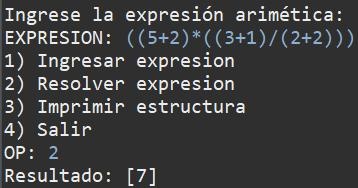
\includegraphics[scale=0.5]{Imagenes/AEA1}
		\hfil
		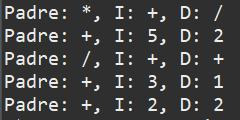
\includegraphics[scale=0.5]{Imagenes/AEA2}
		\caption{De izquierda a derecho, solución de la expresión e impresión del árbol de expresión}
	\end{figure}
	
	\begin{figure}[H]
		\centering
		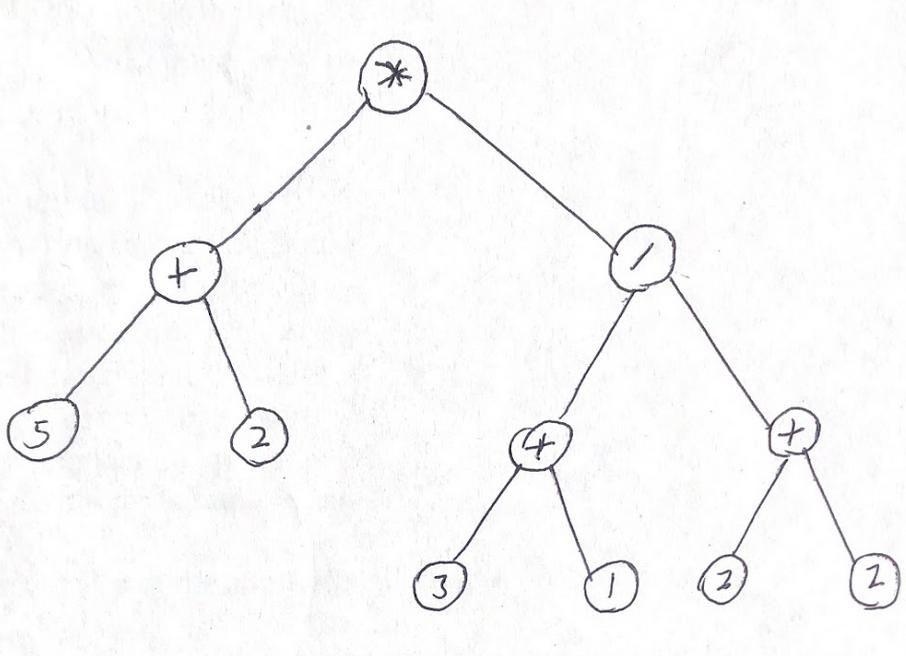
\includegraphics[scale=0.3]{Imagenes/AEA}
		\caption{Representación gráfica del árbol de expresión aritmética correspondiente a "((5+2)*((3+1)/(2+2)))"}
	\end{figure}
	
	Si bien, aunque esta implementación es totalmente mejorable, es una aproximación correcta en el aspecto algorítmico. El problema de esta implementación se encuentra en la lectura de expresiones aritméticas, lo cual tiene que ver más con los aspectos técnicos del lenguaje.
	
	\newpage
	
	\section*{\centering Conclusión}
	
	En general, en este proyecto se pudieron desarrollar y conocer con mayor detalle algunas estructuras de datos basadas en árbol binario que no se vieron a profundidad en durante el curso. El tema de árboles y grafos fue mi favorito del curso, así que disfruté del desarrollo de este proyecto. 
	
	Anteriormente no me había agradado el hecho de no ver estas estructuras de datos con mayor detalle a lo largo del curso, pero durante el desarrollo de este proyecto me di cuenta de que, en realidad, se trata de estructuras complejas que quizás sobrepasan un poco el nivel del curso. Yo desarrollé cada una de las estructuras conforme se solicitaron, es decir, primero realicé el árbol binario autobalanceable, después el montículo, y terminé con árbol de expresión aritmética; y noté que la complejidad de cada estructura fue en aumento. Fue una sorpresa enorme darme cuenta de que, a pesar de que la estructura recién concluida había sido un reto, la siguiente representaba a uno mayor. En sí, todas las estructuras de este proyecto me resultaron bastante complejas, pues tardé muchas horas en desarrollar cada una. 
	
	Considero que algunos aspectos son mejorables, como el enfoque orientado a objetos, o algunos elementos de código que se repiten. Lo que menos me gustó en los resultados es la estructura de árbol de expresiones aritméticas, pues además de que no es tan robusta al momento de recibir expresiones, no puede operar con todos los números enteros. Sin embargo, estoy bastante conforme con los resultados que se entregan porque puedo afirmar que las implementaciones presentes son totalmente de mi autoría, y además son funcionales. 
	
	Por otro lado, este fue el primer (y último) proyecto de la asignatura que realicé de manera individual. Considero que mi forma de trabaja es mejor cuando trabajo sólo, pero sí me hubiera ayudado un poco repartir responsabilidades con alguien más en un proyecto de esta complejidad.
	
	En conclusión, los objetivos del proyecto se cumplieron porque, pese a que el enfoque orientado a objetos es mejorable, se pudieron implementar y comprender algunas de las estructuras de árbol binario más importantes.
	

\end{document}}